\documentclass[xcolor=dvipsnames]{beamer}

\usetheme{AnnArbor}
\usepackage{dsfont}
\usepackage{amsmath}
\usepackage{caption}
\usepackage{hyperref}
\usepackage{xcolor}
\usepackage{color}
\usepackage{commath}
\usepackage{physics}
\usepackage{enumerate}
\usepackage{hyperref}
\usepackage{graphics}
\usepackage{graphicx}
\usepackage[round]{natbib}
\usepackage{subcaption}

%\usepackage[backend=bibtex, style=authoryear-comp]{biblatex}

\setbeamertemplate{bibliography item}{\insertbiblabel}
\beamertemplatenavigationsymbolsempty

\usepackage{filecontents}
\begin{filecontents}{\jobname.bib}
\end{filecontents}
\usepackage[style=authoryear]{biblatex}
\renewcommand*{\nameyeardelim}{\addcomma\addspace}
\addbibresource{\jobname.bib}

\newcommand{\customcite}[1]{\citeauthor{#1} (\citeyear{#1})}

\newtheorem{satz}{Satz}

\setbeamertemplate{footline}[page number]

\usecolortheme{seagull}
\setbeamercolor{frametitle}{fg=blue,bg=White}

%\DeclareMathOperator*{\argmax}{arg\, max}
%\DeclareMathOperator*{\argmin}{arg\, min}
%\setbeamertemplate{section in toc}[sections numbered]
%\setbeamertemplate{subsection in toc}[subsections numbered]
%\AtBeginSection[]
%{
%\begin{frame}
%\frametitle{Überblick}
%\tableofcontents[currentsection]
%\end{frame}
%}
%
%\AtBeginSubsection[
% {\frame<beamer>{\frametitle{Überblick}   
%  \tableofcontents[currentsection,currentsubsection]}}%
%]%
%{
 % \frame<beamer>{ 
 %   \frametitle{Überblick}   
   % \tableofcontents[currentsection,currentsubsection]}
%}

\title{Twitter in the Parliament - A Text-based Analysis of German Political Entities}
%\author{Patrick Schulze}
\date{7. Juli 2020}
\author[author1]{Patrick Schulze, Simon Wiegrebe\\[10mm]{\small Supervisors:\\ Prof. Dr. Christian Heumann, Prof. Dr. Paul W. Thurner}}

\begin{document}

\begin{frame}
\titlepage
\end{frame}

%\begin{frame}
%\frametitle{Überblick}
%\tableofcontents[]
%\end{frame}

\section{Topic Modeling: Motivation and Theory}
\begin{frame}
\frametitle{Topic Modeling: Motivation and Theory}
\framesubtitle{Motivation}
\begin{itemize}
\item bla
\end{itemize}
\end{frame}

\begin{frame}
\frametitle{Topic Modeling: Motivation and Theory}
\framesubtitle{\textit{Structural Topic Model} (STM)}
\begin{itemize}
\item Topic model that incorporates document-level metadata: 
\begin{itemize}
\item \textit{Topical prevalence} covariates $\boldsymbol{X}=[\boldsymbol{x_1}|\dots|\boldsymbol{x_D}]^T \in \mathbb{R}^{D \times P}$
\item Categorical \textit{topical content} variable $\boldsymbol{Y}\in \mathbb{R}^D$ with $A$ levels, i.e., $Y_d \in \{1,\dots,A\}$, for all $d \in \{1,\dots,D\}$
\end{itemize}
\item Generative process for each document $d \in \{1,\dots,D\}$:
\item[] 
\begin{enumerate}[{1)}]
\item Draw $\boldsymbol{\eta}_d \sim \mathcal{N}_{K-1}(\boldsymbol{\Gamma}^T\boldsymbol{x_d}^T, \boldsymbol{\Sigma})$, with $\eta_{d,K}=0$ for model identifiability.
\item Normalize $\boldsymbol{\eta}_d$, for all $k \in \{1,\dots,K\}: \theta_{d,k} = \frac{exp(\eta_{d,k})}{\sum_{j=1}^{K}exp(\eta_{d,j})}$.
\item For each word $n \in \{1,\dots,N_d\}$:
	\begin{enumerate}[{a)}]
    \item Draw topic assignment $\boldsymbol{z}_{d,n} \sim \text{Multinomial}_K(\boldsymbol{\theta}_d)$.
    \item If no topical content variable specified: $w_{d,n} \sim \text{Multinomial}_V(\boldsymbol{\beta}_{d,n})$. 
    \item Otherwise, determine document-specific word distributions $\boldsymbol{B_a} := [\boldsymbol{\beta}^a_1|\dots|\boldsymbol{\beta}^a_K]$ based on $Y_d=a$, for all topics $k \in \{1,\dots,K\}$; select $\boldsymbol{\beta}_{d,n}:=\boldsymbol{B_a}\boldsymbol{z}_d,n}$; and draw word $w_{d,n} \sim \text{Multinomial}_V(\boldsymbol{\beta}_{d,n})$.
	\end{enumerate}
\end{enumerate}
\end{itemize}
\end{frame}

\begin{frame}
\frametitle{Topic Modeling: Motivation and Theory}
\framesubtitle{Graphical Model of the STM}
\begin{itemize}
\item Again, we can visualize the generative process using the representation as a graphical model:
\begin{figure}[h!]
\centering
\hspace*{-1cm}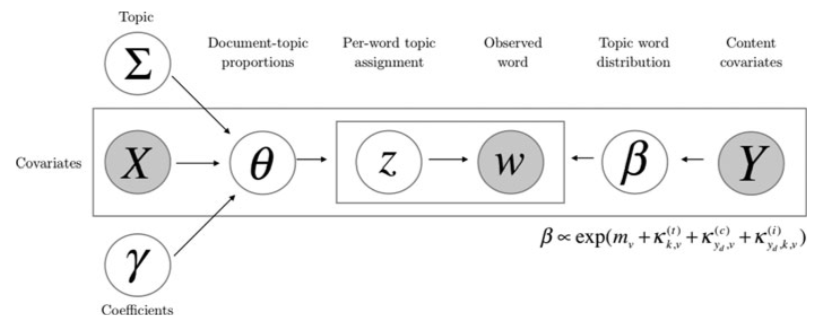
\includegraphics[scale = 0.3]{../../plots/presentation/stm_graphical.png}
\end{figure}
\end{itemize}
\end{frame}

\begin{frame}
\frametitle{Covariate-level Topic Analysis}
\framesubtitle{Overview}
\begin{itemize}
\item Explore estimated topical structure with respect to different dimensions, e.g.\ membership in political party, time, $\dots$
\item Precisely: examine relationship between document-level prevalence covariates $\boldsymbol{x}_d$ and topic proportions $\boldsymbol{\theta}_d$
\item Natural idea: regress topic proportions on prevalence covariates
\begin{itemize}
\item In standard regression analysis, dependent variable is realization of random variable
\item In STM, however, we have access to posterior of topic proportions $\boldsymbol{\theta}_d$
\item If we "na{\"i}vely" use mean/mode of this posterior as dependent variable of regression, much information is lost
\item Solution: perform sampling technique known as "method of composition" in social sciences
\end{itemize}
\item Alternatively: direct assessment of logistic normal distribution with estimated topical prevalence parameters $\hat{\boldsymbol{\Gamma}}$ and $\hat{\boldsymbol{\Sigma}}$
\end{itemize}
\end{frame}

\begin{frame}
\frametitle{Covariate-level Topic Analysis}
\framesubtitle{Method of Composition: Usage within R Package \textit{stm}}
\begin{itemize}
\item Notation:
\begin{itemize}
\item $\boldsymbol{\theta}_{(k)}:=(\theta_{1,k}, \dots, \theta_{D,k})^T \in [0,1]^{D}$: proportion of $k$-th topic for all $D$ documents
\item $q(\boldsymbol{\theta}_{(k)} | \boldsymbol{X}, \boldsymbol{W})$: approximate variational posterior of $\boldsymbol{\theta}_{(k)}$
\item $q(\hat{\boldsymbol{\xi}} | \boldsymbol{X}, \boldsymbol{\theta}_{(k)})$: (normal) distribution of estimated regression coefficients $\hat{\boldsymbol{\xi}}$ from OLS regression $\boldsymbol{\theta}_{(k)} = \boldsymbol{X}\boldsymbol{\xi} + \boldsymbol{\epsilon}$, where $\boldsymbol{\epsilon} \sim \mathcal{N}(0,\sigma^2\boldsymbol{I})$
\end{itemize}
\item Method of composition:
\begin{enumerate}[{1)}]
\item Draw $\boldsymbol{\theta}_{(k)}^* \sim q(\boldsymbol{\theta}_{(k)} | \boldsymbol{X}, \boldsymbol{W})$.
\item Draw $\hat{\boldsymbol{\xi}}^* \sim q(\hat{\boldsymbol{\xi}} | \boldsymbol{X}, \boldsymbol{\theta}_{(k)}^*)$.
\end{enumerate}
\item It then holds that $\hat{\boldsymbol{\xi}}_1^*, \dots, \hat{\boldsymbol{\xi}}_m^*$ is an i.i.d.\ sample from the marginal posterior of regression coefficients
\begin{align*}
q(\boldsymbol{\xi} | \boldsymbol{X}, \boldsymbol{W}) = \int_{\boldsymbol{\theta}_{(k)}} q(\boldsymbol{\xi} | \boldsymbol{X}, \boldsymbol{\theta}_{(k)}) q(\boldsymbol{\theta}_{(k)} | \boldsymbol{X}, \boldsymbol{W}) \text{d} \boldsymbol{\theta}_{(k)} 
\end{align*}
\end{itemize}
\end{frame}

\begin{frame}
\begin{itemize}
\item Problem: OLS regression not suitable for (sampled) proportions, which are restricted to interval (0,1)
\item[$\Rightarrow$] Estimated relationship between proportions and prevalence covariates might involve negative estimated proportions
\end{itemize}
\frametitle{Covariate-level Topic Analysis}
\framesubtitle{Method of Composition: Usage within R Package \textit{stm}}
  \begin{figure}[h!]
  \centering
  \captionsetup{justification=centering,margin=2cm}
  \begin{subfigure}[b]{0.4\linewidth}
    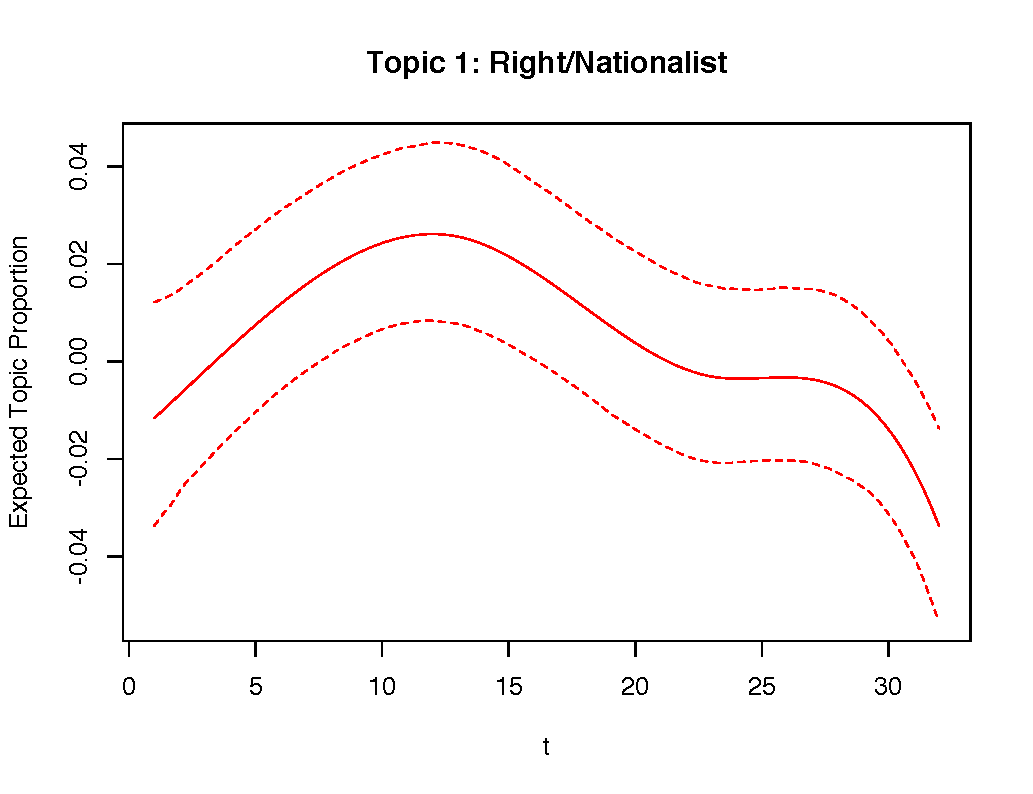
\includegraphics[width=\linewidth]{../../plots/presentation/estEffect_topic1.pdf}
  \end{subfigure}
  \begin{subfigure}[b]{0.4\linewidth}
    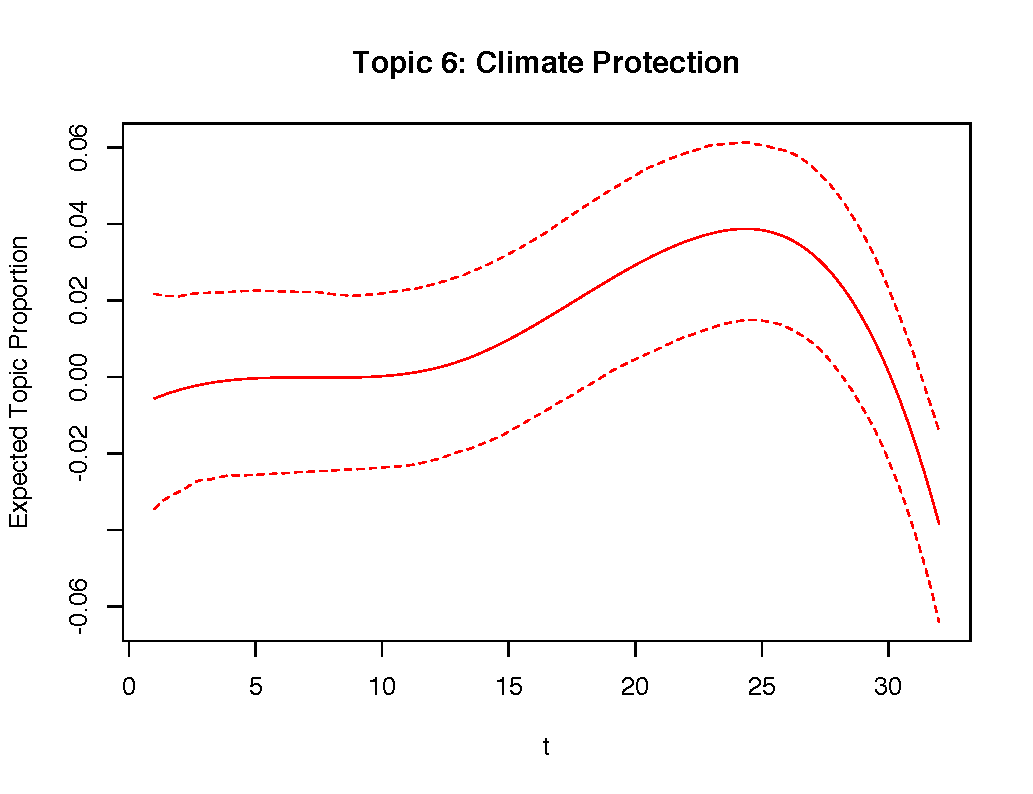
\includegraphics[width=\linewidth]{../../plots/presentation/estEffect_topic6.pdf}
  \end{subfigure}
\end{figure}
\end{frame}

\begin{frame}
\frametitle{Covariate-level Topic Analysis}
\framesubtitle{Method of Composition: Extension of existing approach}
\begin{itemize}
\item Instead of OLS regression, we can use a beta regression or a quasibinomial GLM (both with logit-link) to adequately model proportions
\item In this case, regression coefficients are \textit{asymptotically} normally distributed
\end{itemize}
\begin{figure}[h!]
  \centering
  \captionsetup{justification=centering,margin=2cm}
  \begin{subfigure}[b]{0.4\linewidth}
    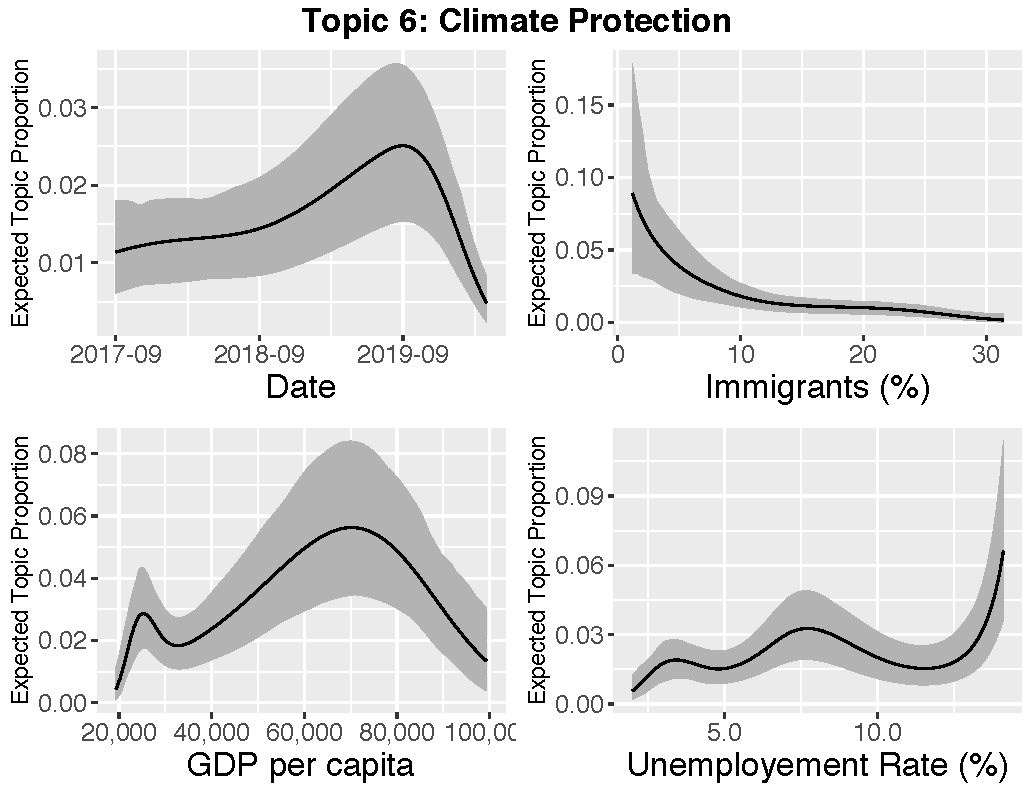
\includegraphics[width=\linewidth]{../../plots/presentation/quasi_t6_cont.pdf}
  \end{subfigure}
  \begin{subfigure}[b]{0.4\linewidth}
    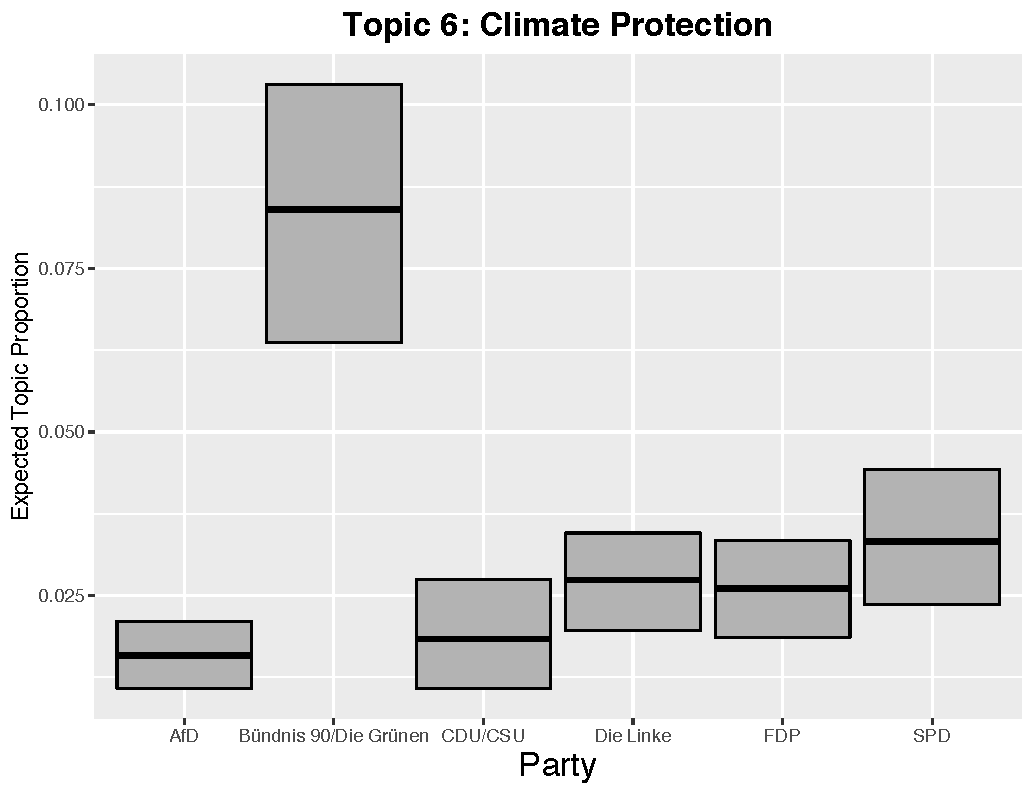
\includegraphics[width=\linewidth]{../../plots/presentation/quasi_t6_cat.pdf}
  \end{subfigure}
\end{figure}
\end{frame}

\begin{frame}
\frametitle{Covariate-level Topic Analysis}
\framesubtitle{Problem: Univariate Modeling of Proportions}
\begin{itemize}
\item Remember, by assumption: $\boldsymbol{\theta}_d \sim \text{LogisticNormal}(\boldsymbol{\Gamma}^T\boldsymbol{x}_d^T, \boldsymbol{\Sigma})$
\item Logistic normal distribution assumes high dependence among individual components
\item However, regression within method of composition uses \textit{univariate} k-th topic proportion as dependant variable 
\item Problem with this approach: dependence among components neglected $\Rightarrow$ especially uncertainty estimates are unrealistic
\end{itemize}
\end{frame}

\begin{frame}
\frametitle{Covariate-level Topic Analysis}
\framesubtitle{Multivariate Modeling via Logistic Normal Distribution}
\begin{itemize}
\item Inference within STM involves finding estimates $\hat{\boldsymbol{\Gamma}}$ and $\hat{\boldsymbol{\Sigma}}$
\item Idea: plug estimates into logistic normal distribution $\Rightarrow$ for a given covariate value $\boldsymbol{x}^*_d$, "predict" topic proportion as
$\boldsymbol{\theta}^*_d \sim \text{LogisticNormal}(\hat{\boldsymbol{\Gamma}}^T(\boldsymbol{x}_d^*)^T, \hat{\boldsymbol{\Sigma}})$
\item Ideally, we would apply fully Bayesian approach and sample from (variational) posterior of $\boldsymbol{\Gamma}$ (and update $\boldsymbol{\Sigma}$, which is obtained via MLE) $\Rightarrow$ "Predictive Posterior" of topic proportions
\item However, output obtained using R package \textit{stm} does not allow for simple implementation of such a procedure (i.e., sampling from variational posterior of $\boldsymbol{\Gamma}$ and updating $\boldsymbol{\Sigma}$); yet, possible in theory!
\end{itemize}
\end{frame}

\begin{frame}
\begin{itemize}
\item Still, our results suggest a high discrepancy between:
\begin{itemize}
\item Distribution of topic proportions assumed in generative process of STM
\item Impression we gain of this distribution via separate modeling of topics.
\end{itemize}
\item Fully Bayesian approach would most likely yield even higher uncertainty
\end{itemize}
\frametitle{Covariate-level Topic Analysis}
\framesubtitle{Multivariate Modeling via Logistic Normal Distribution}
\begin{figure}[h!]
  \centering
  \captionsetup{justification=centering}
  \begin{subfigure}[b]{0.4\linewidth}
    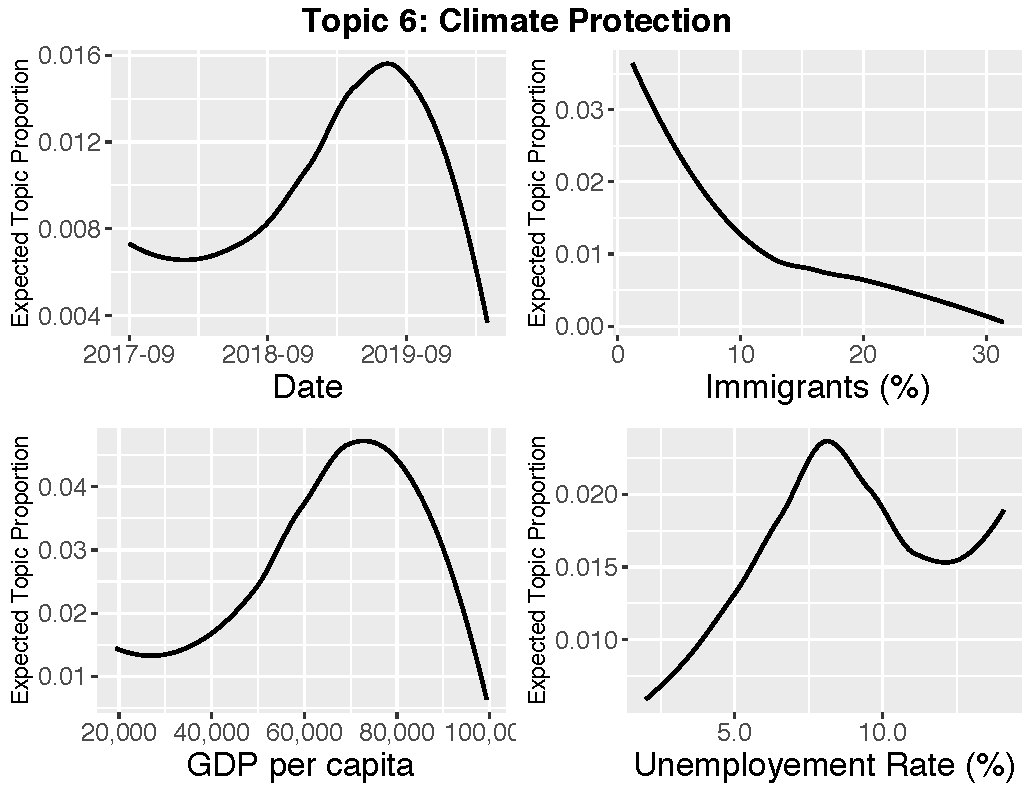
\includegraphics[width=\linewidth]{../../plots/presentation/direct_t6_without_credible.pdf}
  \end{subfigure}
  \begin{subfigure}[b]{0.4\linewidth}
    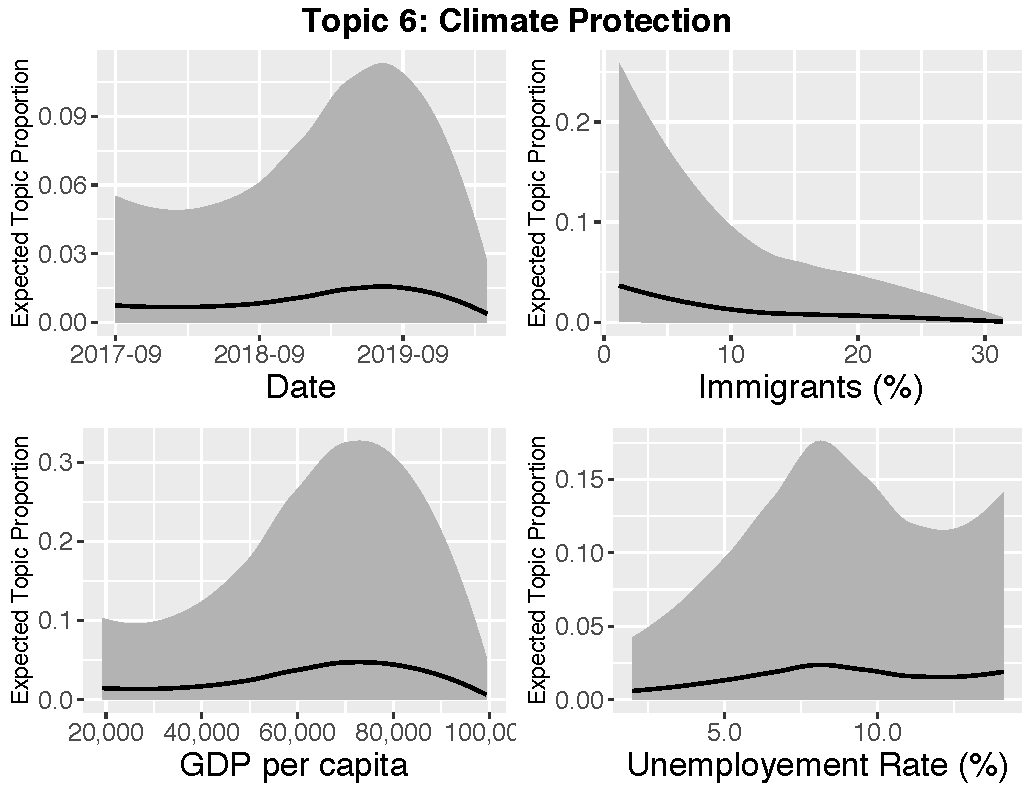
\includegraphics[width=\linewidth]{../../plots/presentation/direct_t6_with_credible.pdf}
  \end{subfigure}
\end{figure}
\end{frame}

\begin{frame}
\frametitle{Causal Inference}
\framesubtitle{Correlation vs. Causality}
\begin{itemize}
\item In previous section: assessment of relationship between metadata and topic proportions
\item As stated, framework should be used to \textit{explore} topics with respect to different dimensions
\item In particular, \textit{causal} interpretation of results is generally not justified ("correlation vs. causality")
\item When making causal inference, we have to consider that topic proportions are \textit{latent} variables 
\item Possible solution: conduct a train-test split
\end{itemize}
\end{frame}

\begin{frame}
\frametitle{Causal Inference}
\framesubtitle{Identification Problem and Overfitting}
\begin{itemize}
\item Assume there are two groups, a treatment group and a control group
\item Aside from treatment, individuals from both groups are similar
\item Objective: quantify treatment effect, in our case effect of treatment on prevalence of specific topic.
\item Necessary assumption: response of an individual depends only on treatment of this individual
\item \textit{Identification problem}: estimating topic model to discover latent topic proportions can introduce additional dependency among individuals $\Rightarrow$ response of each individual is \textit{not} only determined by treatment of that individual!
\item \textit{Overfitting}: fitted topic model might mistake noise for patterns in some way $\Rightarrow$ response again not solely determined by treatment of an individual, but additionally by specific characteristics of other individuals.
\end{itemize}
\end{frame}


\begin{frame}
\frametitle{Causal Inference}
\framesubtitle{Train-test split}
\begin{itemize}
\item Idea: split data $\mathcal{D}$ into training set $\mathcal{D}_{\text{train}}$ and test set $\mathcal{D}_{\text{test}}$. 
\item Training set $\mathcal{D}_{\text{train}}$ used to determine a model that infers latent topic proportions from a given text 
\item Test set $\mathcal{D}_{\text{test}}$ used in order to assess relation between \textit{predicted} test set topic proportions and test set prevalence covariates.
\item Solves identification problem: model used for prediction is determined by training set observations $\Rightarrow$ treatment of test set observations not dependent on other individuals' treatment from test set. 
\item Overfitting also solved: noise from training set is very unlikely to be replicated on test set
\end{itemize}
\end{frame}

\begin{frame}
\frametitle{Causal Inference}
\framesubtitle{Implementation within the STM}
\begin{itemize}
\item Input documents, i.e., words and metadata from the training set $\mathcal{D}_{\text{train}}$, and obtain estimates $(\hat{\boldsymbol{\beta}}_{\text{train}}, \hat{\boldsymbol{\Gamma}}_{\text{train}}, \hat{\boldsymbol{\Sigma}}_{\text{train}})$ using the STM
\item Then, estimate (variational) posterior of test set topic proportions, conditional on the model parameters $(\hat{\boldsymbol{\beta}}_{\text{train}}, \hat{\boldsymbol{\Gamma}}_{\text{train}}, \hat{\boldsymbol{\Sigma}}_{\text{train}})$ from training set $\mathcal{D}_{\text{train}}$ as well as words $\boldsymbol{W}_{\text{test}}$ from test set $\mathcal{D}_{\text{test}}$
\item Estimation of (variational) posterior conditional on data and training set parameters occurs via E-step of (variational) EM algorithm
\item Benefit of using the STM: covariate information from training set directly used to predict topic proportions on test set
\item Important: Covariate information from test set must not be used! Otherwise, for two documents from test set with exact same words, different topic proportions are predicted if prevalence covariates differ. However, in such a case causal effect should to be zero.
\end{itemize}
\end{frame}

\begin{frame}
\frametitle{Causal Inference}
\framesubtitle{Results}
\begin{figure}[h!]
  \centering
  \captionsetup{justification=centering}
  \begin{subfigure}[b]{0.49\linewidth}
    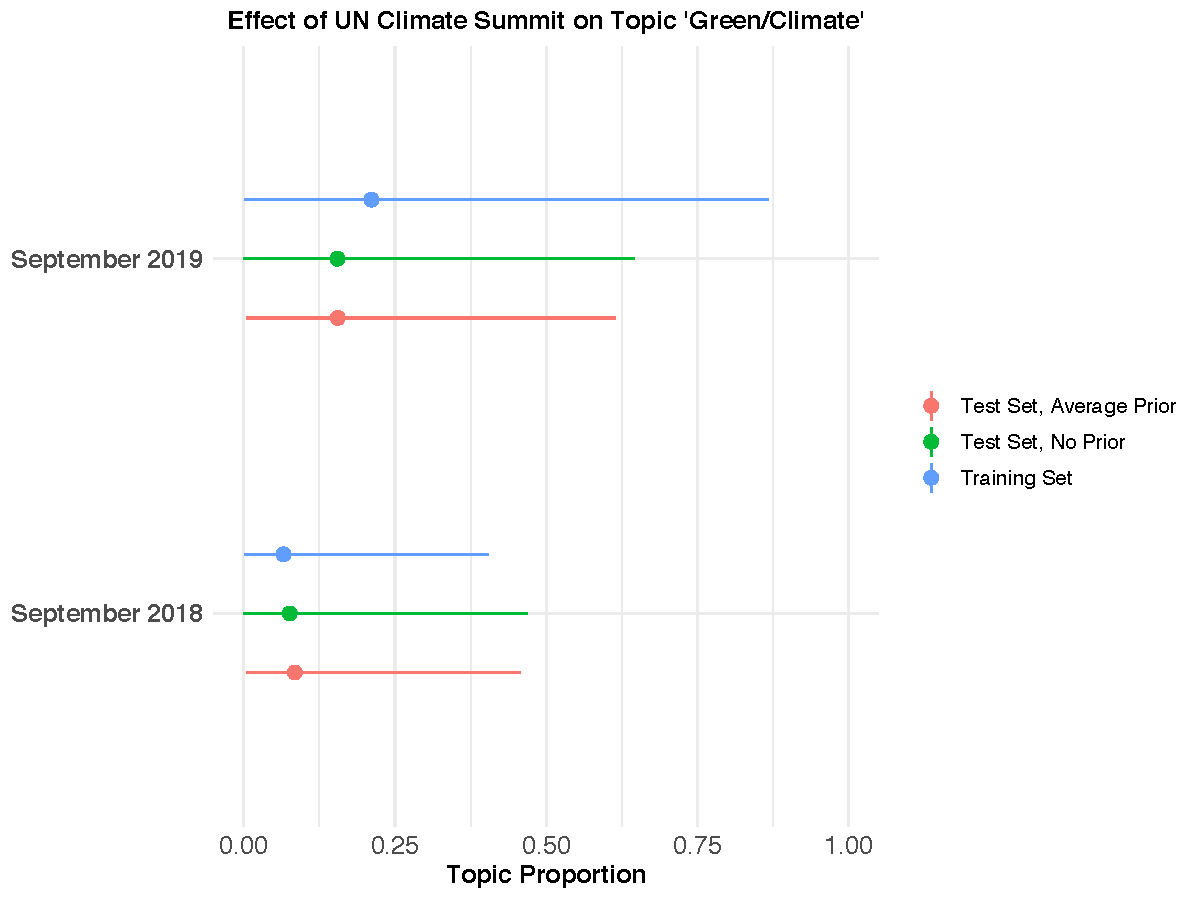
\includegraphics[width=\linewidth]{../../plots/presentation/climate_summit_props.pdf}
  \end{subfigure}
  \begin{subfigure}[b]{0.49\linewidth}
    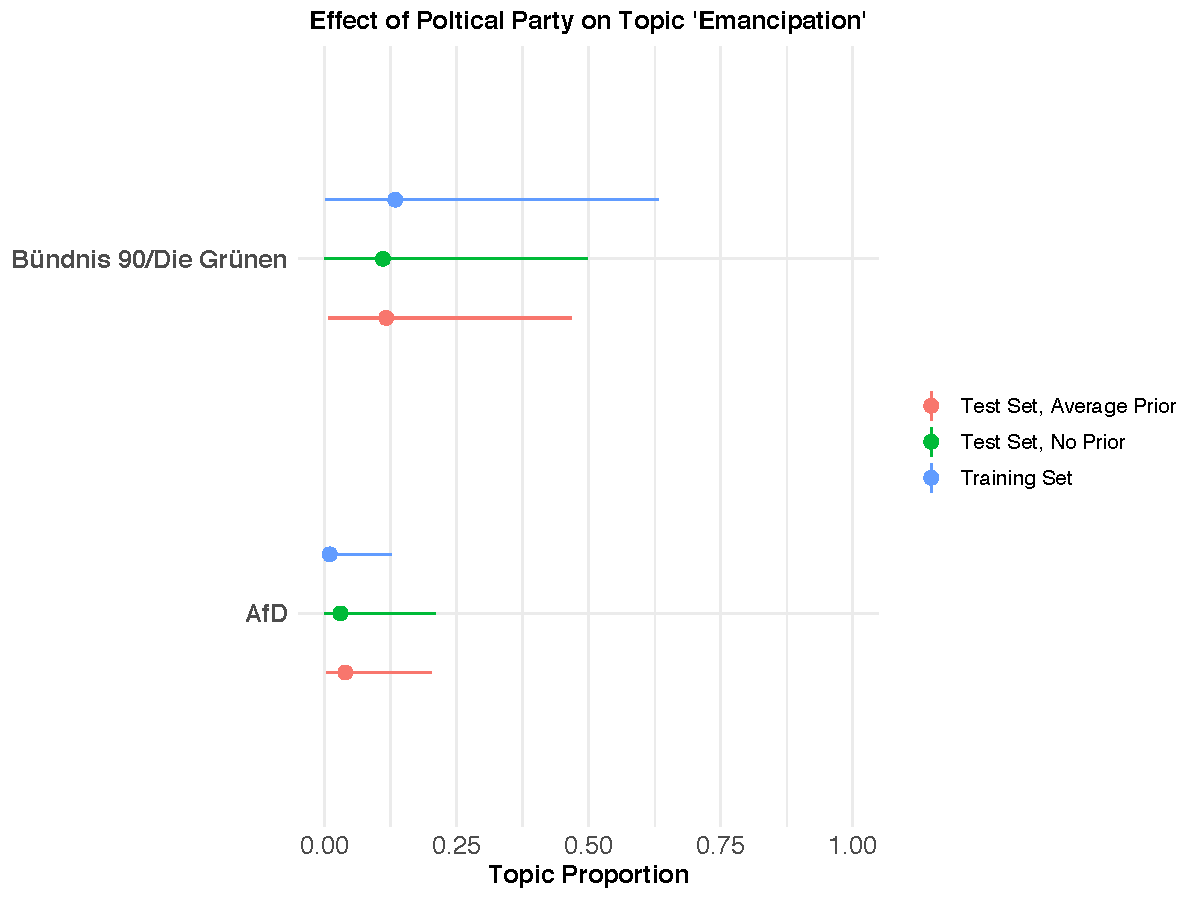
\includegraphics[width=\linewidth]{../../plots/presentation/emancipation_props.pdf}
  \end{subfigure}
\end{figure}
\end{frame}

\begin{frame}
\frametitle{Causal Inference}
\framesubtitle{Results}
\begin{itemize}
\item UN Climate Action Summit 2019 was held on September 23, 2019
\item As observed, topic associated with climate issues was discussed to much larger extent during that time than the year before
\item While MAP estimates for different prior specifications on test set are rather similar, estimated effect for training data is much larger
\item For effect of political party on topic labelled as 'Emancipation', we find similar results: average difference of estimated topic proportions between both parties is larger for the training data
\item Further, note that credible intervals on the training data differ compared to credible intervals on the test data in both cases.
\end{itemize}
\end{frame}

\begin{frame}
\begin{itemize}
\item To estimate the treatment effect, we determine the average difference of predicted topic proportions between both groups:
\begin{figure}[h!]
  \centering
  \captionsetup{justification=centering,margin=2cm}
  \begin{subfigure}[b]{0.4\linewidth}
    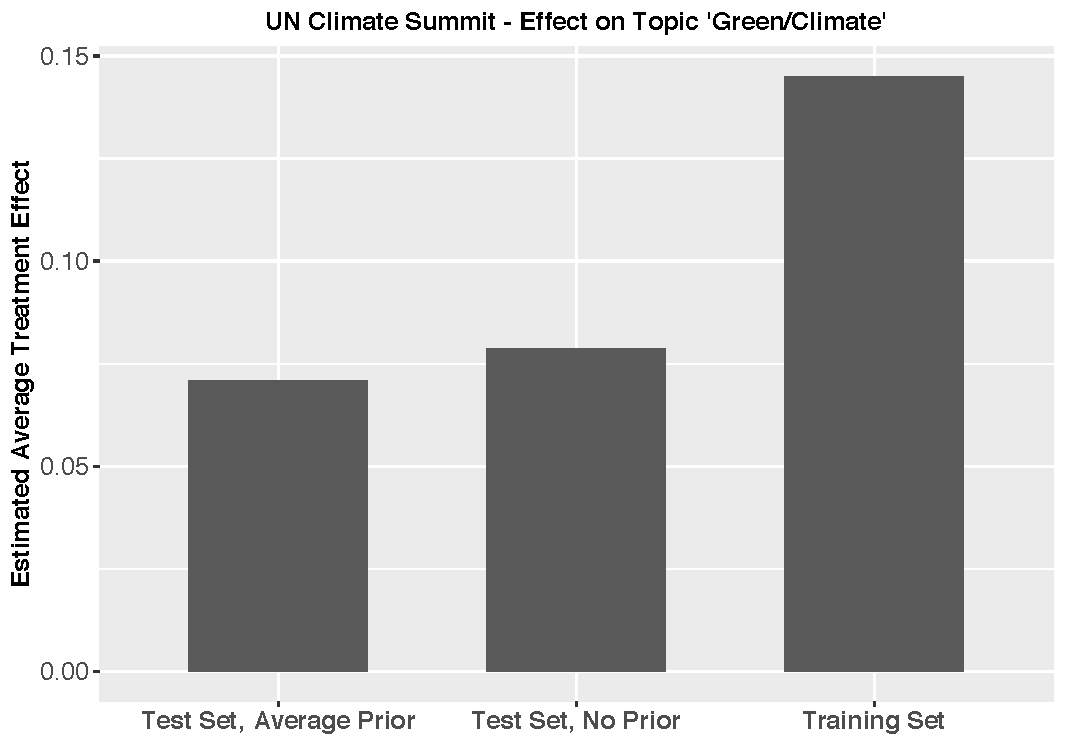
\includegraphics[width=\linewidth]{../../plots/presentation/climate_summit_ate.pdf}
  \end{subfigure}
  \begin{subfigure}[b]{0.4\linewidth}
    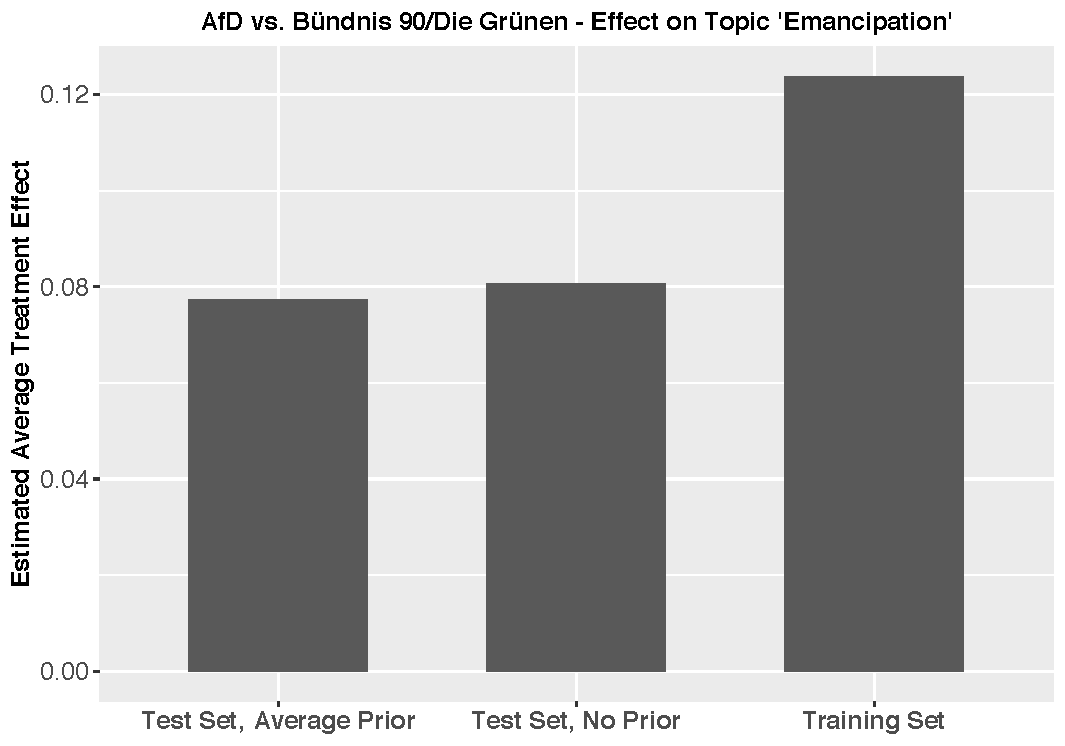
\includegraphics[width=\linewidth]{../../plots/presentation/emancipation_ate.pdf}
  \end{subfigure}
\end{figure}
\item In both cases treatment effect is larger if "na{\"i}vely" estimated solely on training data!
\end{itemize}
\end{frame}

\begin{frame}
\frametitle{Bibliography}
\printbibliography
\end{frame}
\end{document}